%%%%%%%%%%%%%%%%%%%%%%%%%%%%%%%%%%%%%%%%%
% Short Sectioned Assignment
% LaTeX Template
% Version 1.0 (5/5/12)
%
% This template has been downloaded from:
% http://www.LaTeXTemplates.com
%
% Original author:
% Frits Wenneker (http://www.howtotex.com)
%
% License:
% CC BY-NC-SA 3.0 (http://creativecommons.org/licenses/by-nc-sa/3.0/)
%
%%%%%%%%%%%%%%%%%%%%%%%%%%%%%%%%%%%%%%%%%

%----------------------------------------------------------------------------------------
%	PACKAGES AND OTHER DOCUMENT CONFIGURATIONS
%----------------------------------------------------------------------------------------

\documentclass[paper=a4, fontsize=11pt]{scrartcl} % A4 paper and 11pt font size
\usepackage{url}
\usepackage{gensymb}
\usepackage{csquotes}
\usepackage{graphics}
\usepackage{graphicx}
\usepackage{wrapfig}
\usepackage{subfig}
\usepackage{float}
\usepackage[T1]{fontenc} % Use 8-bit encoding that has 256 glyphs
\usepackage{fourier} % Use the Adobe Utopia font for the document - comment this line to return to the LaTeX default
\usepackage[english]{babel} % English language/hyphenation
\usepackage{amsmath,amsfonts,amsthm} % Math packages

\usepackage{lipsum} % Used for inserting dummy 'Lorem ipsum' text into the template

\usepackage{sectsty} % Allows customizing section commands
\allsectionsfont{\centering \normalfont\scshape} % Make all sections centered, the default font and small caps

\usepackage{fancyhdr} % Custom headers and footers
\pagestyle{fancyplain} % Makes all pages in the document conform to the custom headers and footers
\fancyhead{} % No page header - if you want one, create it in the same way as the footers below
\fancyfoot[L]{} % Empty left footer
\fancyfoot[C]{} % Empty center footer
\fancyfoot[R]{\thepage} % Page numbering for right footer
\renewcommand{\headrulewidth}{0pt} % Remove header underlines
\renewcommand{\footrulewidth}{0pt} % Remove footer underlines
\setlength{\headheight}{13.6pt} % Customize the height of the header

\numberwithin{equation}{section} % Number equations within sections (i.e. 1.1, 1.2, 2.1, 2.2 instead of 1, 2, 3, 4)
\numberwithin{table}{section} % Number tables within sections (i.e. 1.1, 1.2, 2.1, 2.2 instead of 1, 2, 3, 4)

\setlength\parindent{0pt} % Removes all indentation from paragraphs - comment this line for an assignment with lots of text

%----------------------------------------------------------------------------------------
%	TITLE SECTION
%----------------------------------------------------------------------------------------

\newcommand{\horrule}[1]{\rule{\linewidth}{#1}} % Create horizontal rule command with 1 argument of height

\title{	
\normalfont \normalsize 
\textsc{Final Report\\Data Mining, Spring 2017\\University of Utah} \\ [25pt] % Your university, school and/or department name(s)
\horrule{0.5pt} \\[0.4cm] % Thin top horizontal rule
\huge Ride Hailing Supply and Demand Forecasting using Didi-Tech Dataset  % The assignment title
\horrule{2pt} \\[0.5cm] % Thick bottom horizontal rule
}

\author{Kimberly Williamson, Gopal Menon} % Your name

\date{\normalsize\today} % Today's date or a custom date

\begin{document}

\maketitle % Print the title

%----------------------------------------------------------------------------------------
%	PROBLEM 1
%----------------------------------------------------------------------------------------

\section{Problem and Motivation}
Didi Chuxing is the leading ride hailing company in China and processes over $11$ million trips, plans over $9$ billion routes and collects over $50$TB of data per day. They organized a worldwide algorithm challenge in the year $2016$ \cite{DidiPage} for forecasting ride supply and demand. We used the $2016$ Didi algorithm competition dataset to try and forecast taxi trip supply and demand for any given date, time, and location using regression models covered in the Data Mining 2017 Spring semester at the School of Computing of the University of Utah.

%------------------------------------------------
\section{Ride Hailing Data}

\subsection{Data format conversion}

In order to run the regression models, the categorical values in the Didi algorithm competition dataset needed to be converted into a regression friendly format. Depending on the type of categorical value, the new values are lists that consist of $0$ values when the category is not present in an order and $1$ or a count when the category is present in the order.

\subsection{Data format details}

We have converted the data into a format that can be used by the regression models. The input to the regression consists of:
\begin{itemize}
\item An order key, comprised of the categorical values for start district, destination district and order time
\item An order value consisting of
\begin{itemize}
\item Traffic and points of interest for the start and destination districts
\item Weather at the time of the order
\item The value that needs to be predicted, which is the median order price or the number of orders
\end{itemize}
\end{itemize}

With the input data created, we have experimented with multiple regression models.

\subsection{Data Size}

\begin{figure}[!htb]
\centering
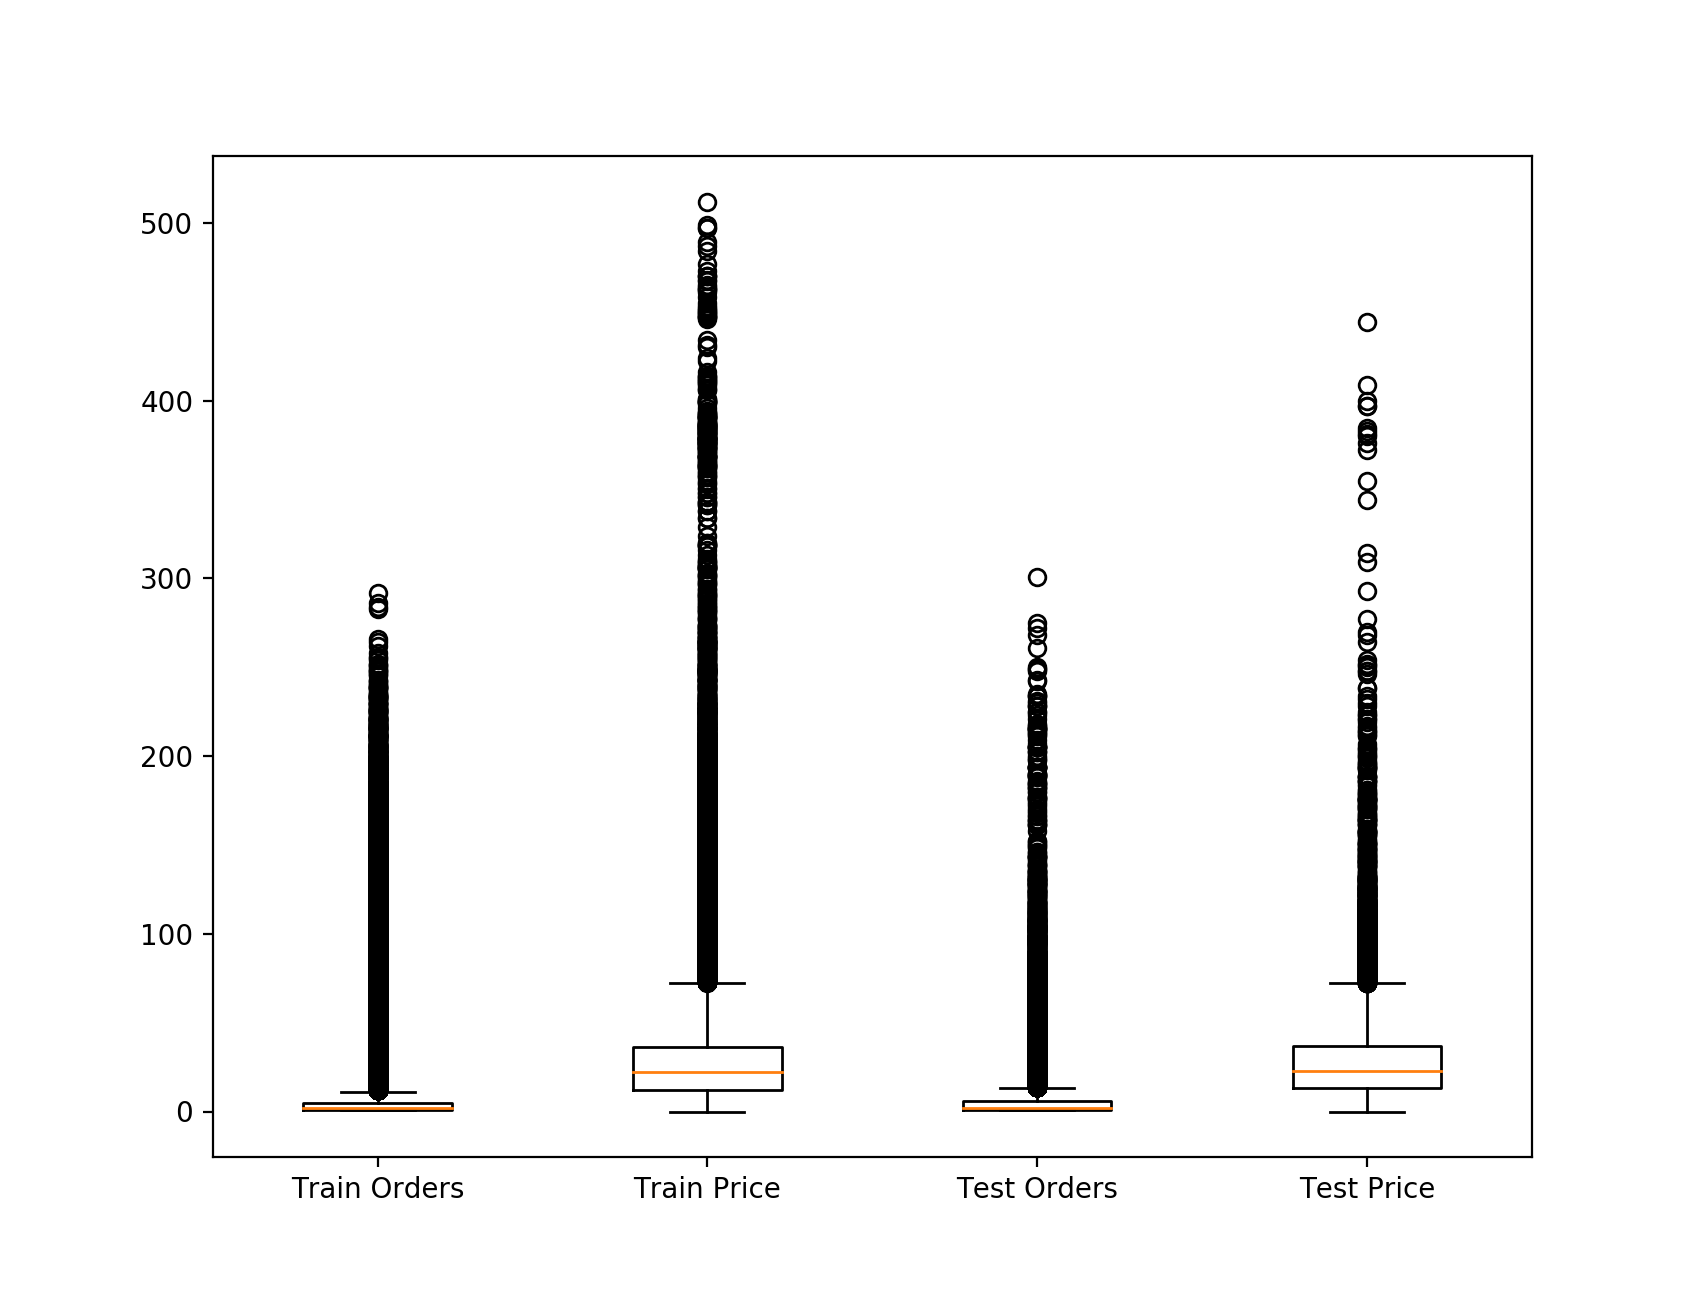
\includegraphics[width=3in]{figures/boxplots.png}
\caption{Box and whisker data plots.}
\label{boxplots}
\end{figure}


\begin{figure}[!htb]
\centering
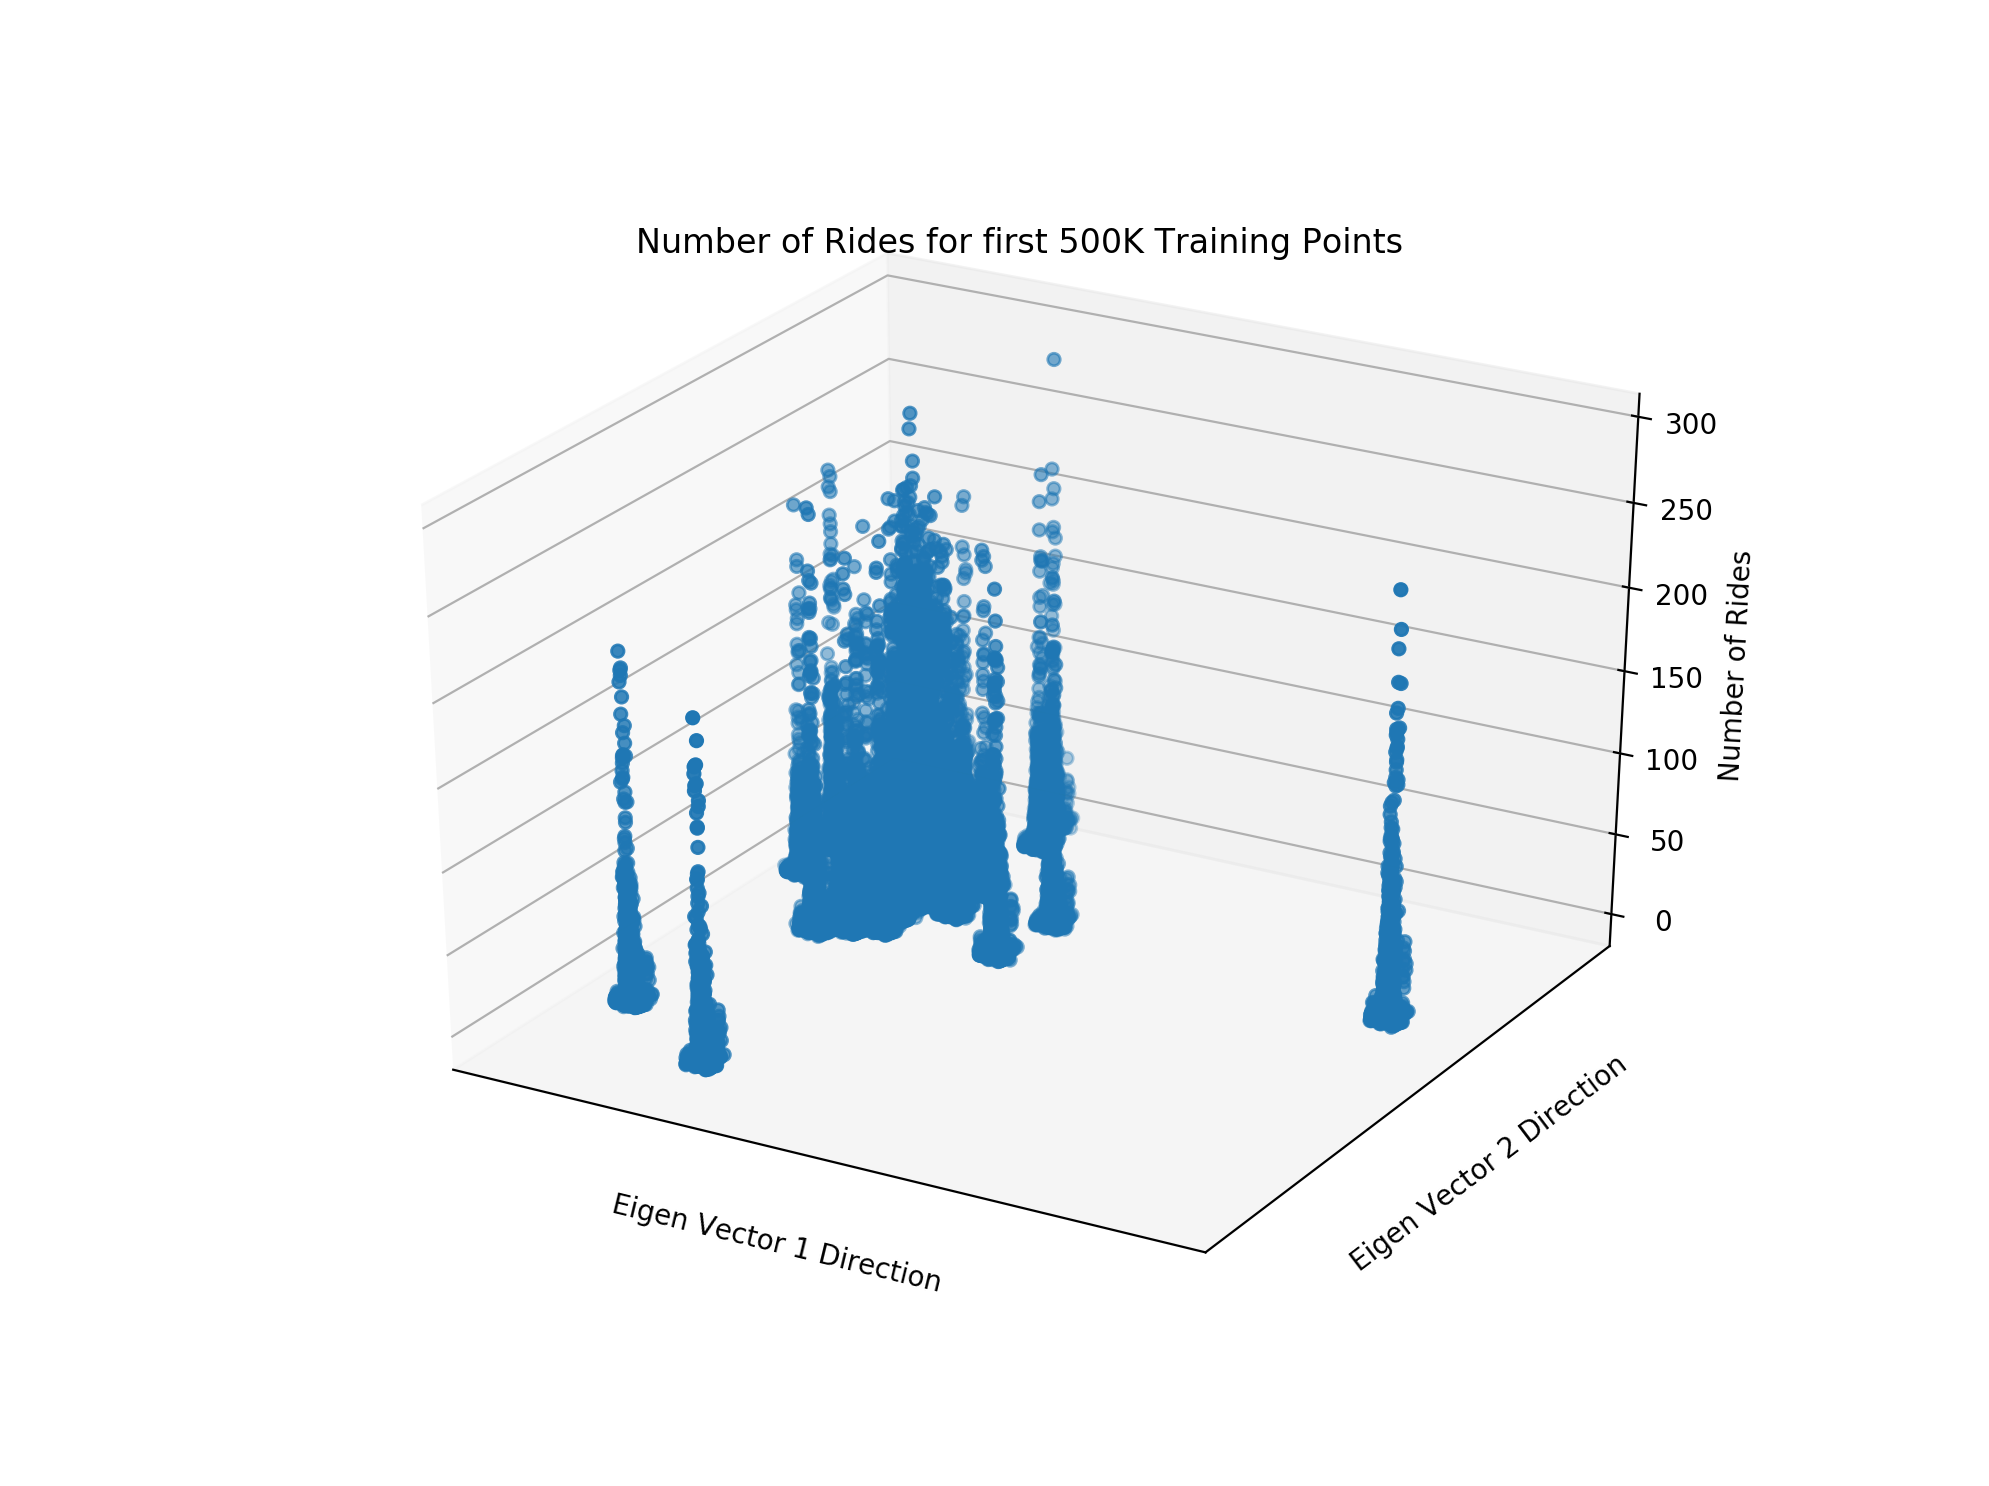
\includegraphics[width=3in]{figures/Rides3DScatter.png}
\caption{Number of rides scatter plot.}
\label{rides}
\end{figure}
We have $1.3$ million rows in our training data consisting of ride hailing orders. When we took into consideration, only those orders where the start and end districts have data for traffic and places of interest, the number of training rows were reduced to $921,000$.

%------------------------------------------------
\section{Key Idea}

The start and end ride locations, driver id, passenger id and points of interest have all been anonymized in the ride hailing data. However we were hopeful that using the regression techniques, that would be able to extract patterns from the data, we could make accurate predictions. We were expecting some sort of correlation between the start and end locations, weather, time, points of interest and the values to be predicted - the number of rides and the price.\\

Although we did not expect the number of rides and the price to have a linear relationship with the ride features, we planned to start with linear regression and then move on to non-linear prediction models for better accuracy. The Python library scikit-Learn \cite{sklearn} was used for running regressions.

%------------------------------------------------
\section{Prediction Accuracy}

\begin{figure}[!htb]
\centering
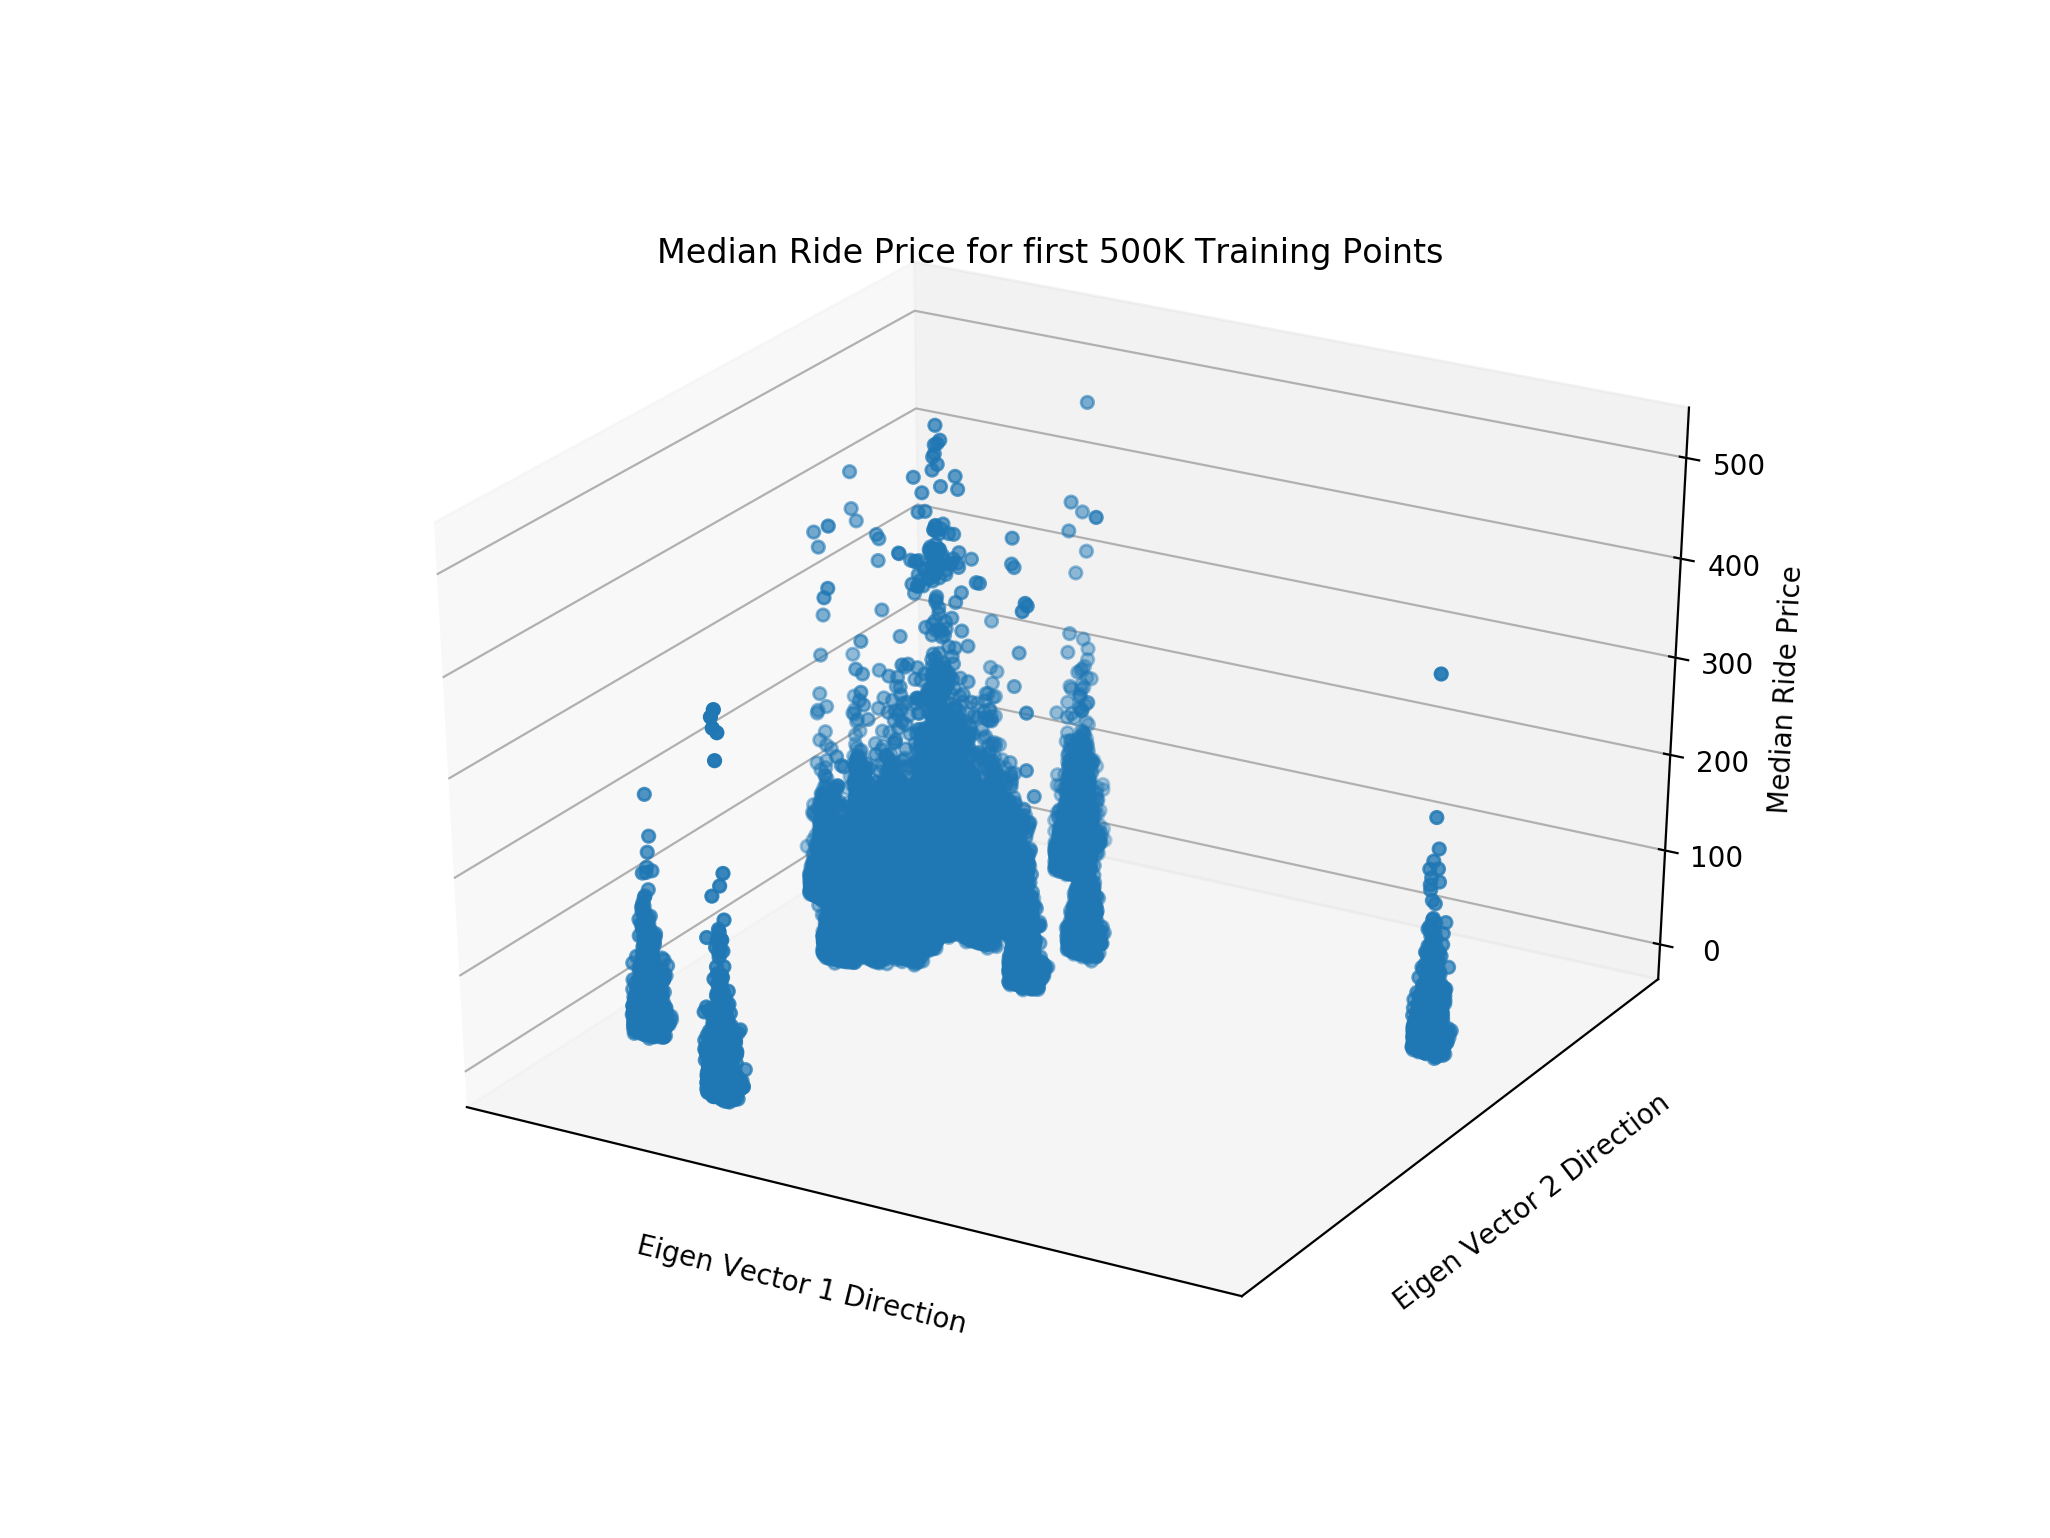
\includegraphics[width=3in]{figures/OrderPrice3DScatter.png}
\caption{Order Price Scatter Plot.}
\label{price}
\end{figure}

    \begin{table}[!h] 
    \centering
    \caption{Regression Results for predicting number of rides}
    \label{results}
    \begin{tabular}{|l|r|}
      \hline
   Regression Type  & Mean Squared Error \\
      \hline      
      Linear using Stochastic Gradient Descent&   $245.50$ \\
      \hline      
      Gradient Boosting using features based on top $10$ eigen vectors &    $285.97$    \\
      \hline
      Ridge Regression using features based on top $10$ eigen vectors&    $293.83$    \\
      \hline
      Lasso Regression using features based on top $10$ eigen vectors&    $293.83$    \\
      \hline
     Polynomial degree 2 regression using features based on top $10$ eigen vectors &    $2.34\times10^{53}$    \\
      \hline
     Polynomial degree 3 regression using features based on top $10$ eigen vectors &    $3.53\times10^{73}$    \\
      \hline
     Polynomial degree 4 regression using features based on top $10$ eigen vectors &    $9.31\times10^{93}$    \\
      \hline
      Gaussian Kernel Regression &    $376.90$    \\
      \hline
    \end{tabular}
    \end{table}

\begin{figure}[!htb]
\centering
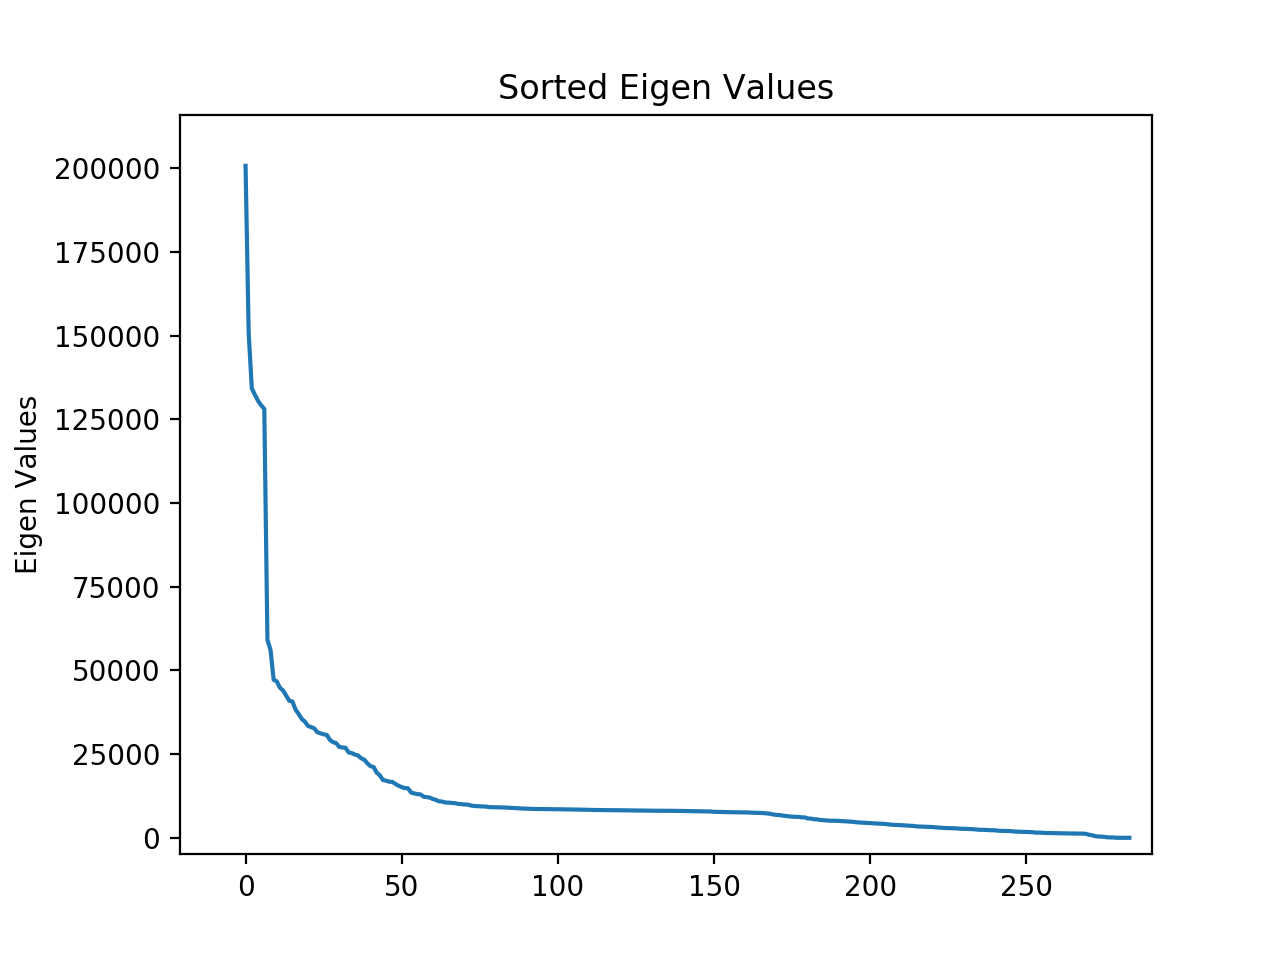
\includegraphics[width=4in]{figures/EigenValues.png}
\caption{Sorted eigen values.}
\label{eigen10}
\end{figure}

The prediction accuracy results for number of rides is shown in table \ref{results}. The regression was run without the data for traffic, weather and points of interest as results were more accurate without this data. The least error was for linear regression using stochastic gradient descent. The results from Guassian Kernel Regression were not very accurate either. The reason was probably that since the start and end locations had been anonymized, we did not have a way to compute a distance between two vectors. If we had this data, the kernel regression results would have been more accurate. We were hoping to get better results using non-linear regression, but the results were surprisingly worse than those for linear regression. We used the first ten eigen vectors for dimensionality reduction as we found that most of the information was encapsulated in these. This is shown in figure \ref{eigen10}.
%------------------------------------------------
\section{Patterns in Ride Hailing Data}

\begin{figure}[!htb]
\centering
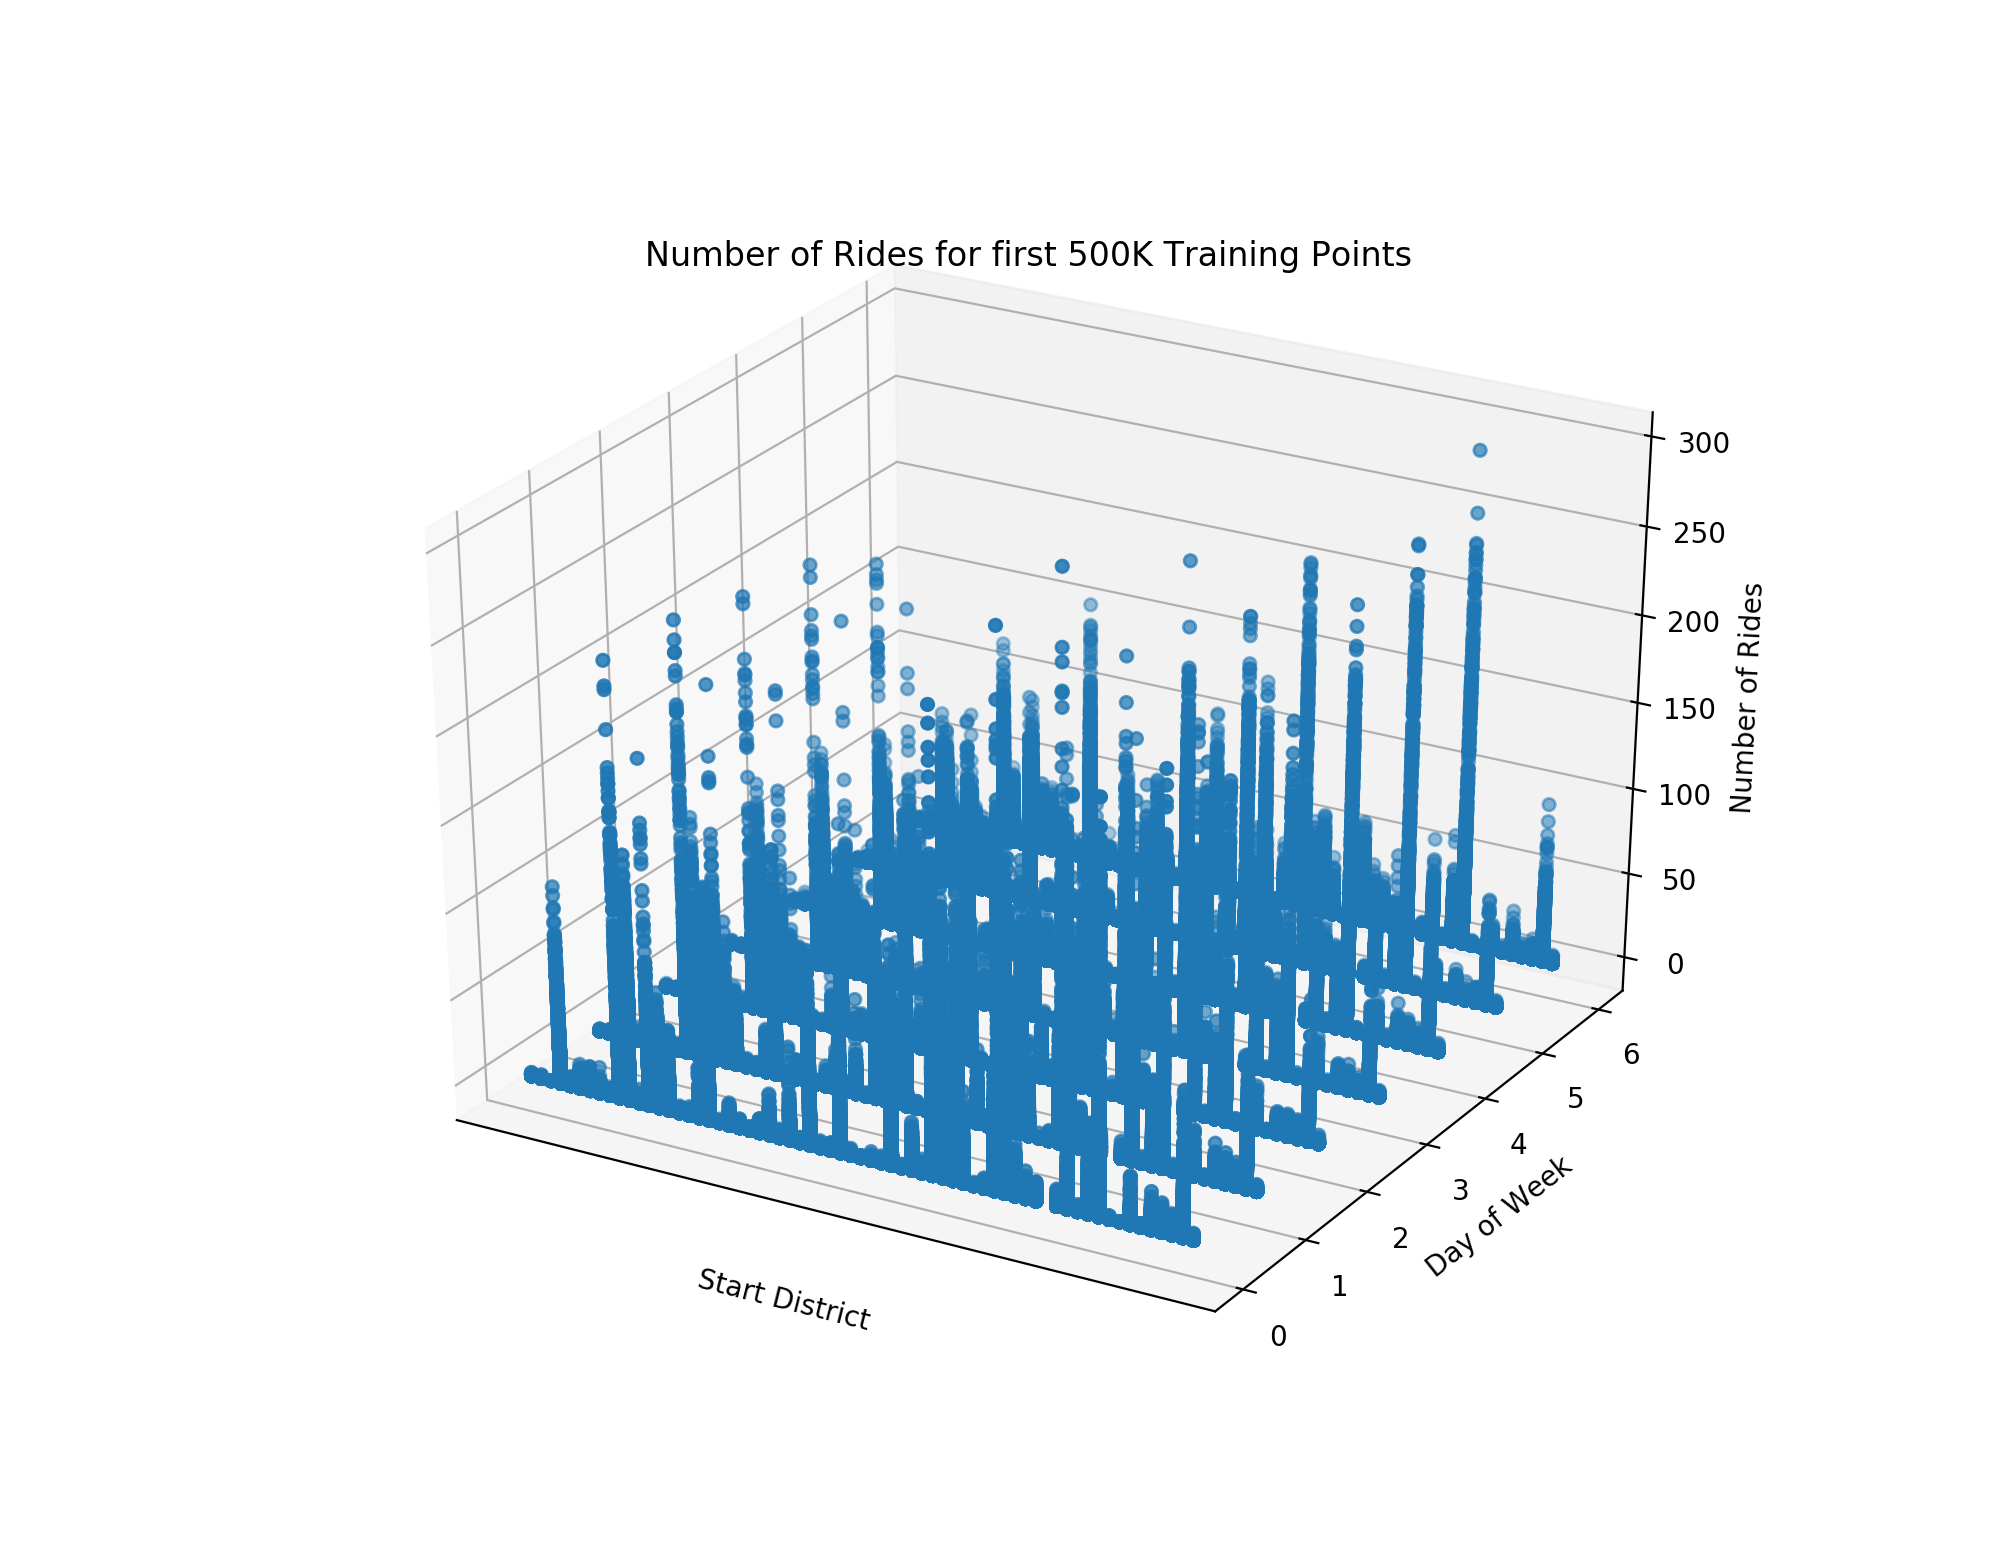
\includegraphics[width=3in]{figures/Ridesfordistrictsandweekdays3DScatter.png}
\caption{Number of rides scatter plot for start district and week day.}
\label{rides2}
\end{figure}

Since we were not getting good results, we decided to see what the data looks like and plotted box and whisker plots for the data. These plots are shown in figure \ref{boxplots} and seem to suggest that there are a lot of outliers. The outliers are usually computed using the inter-quartile distance between the first and third quartiles and using that figure to include elements that are up to $1.5$ times the inter-quartile distance on either side. Elements outside these limits are marked as outliers. However it is doubtful that these are outliers since it is actual data and the reported number of outliers is large.  \\

We next looked at clustering methods to determine and filter out outliers.  After experimenting with a couple of methods with no improvement in the mean squared error, we confirmed our previous theory that the identified outliers are most likely not true outliers. \\

\begin{figure}[!htb]
\centering
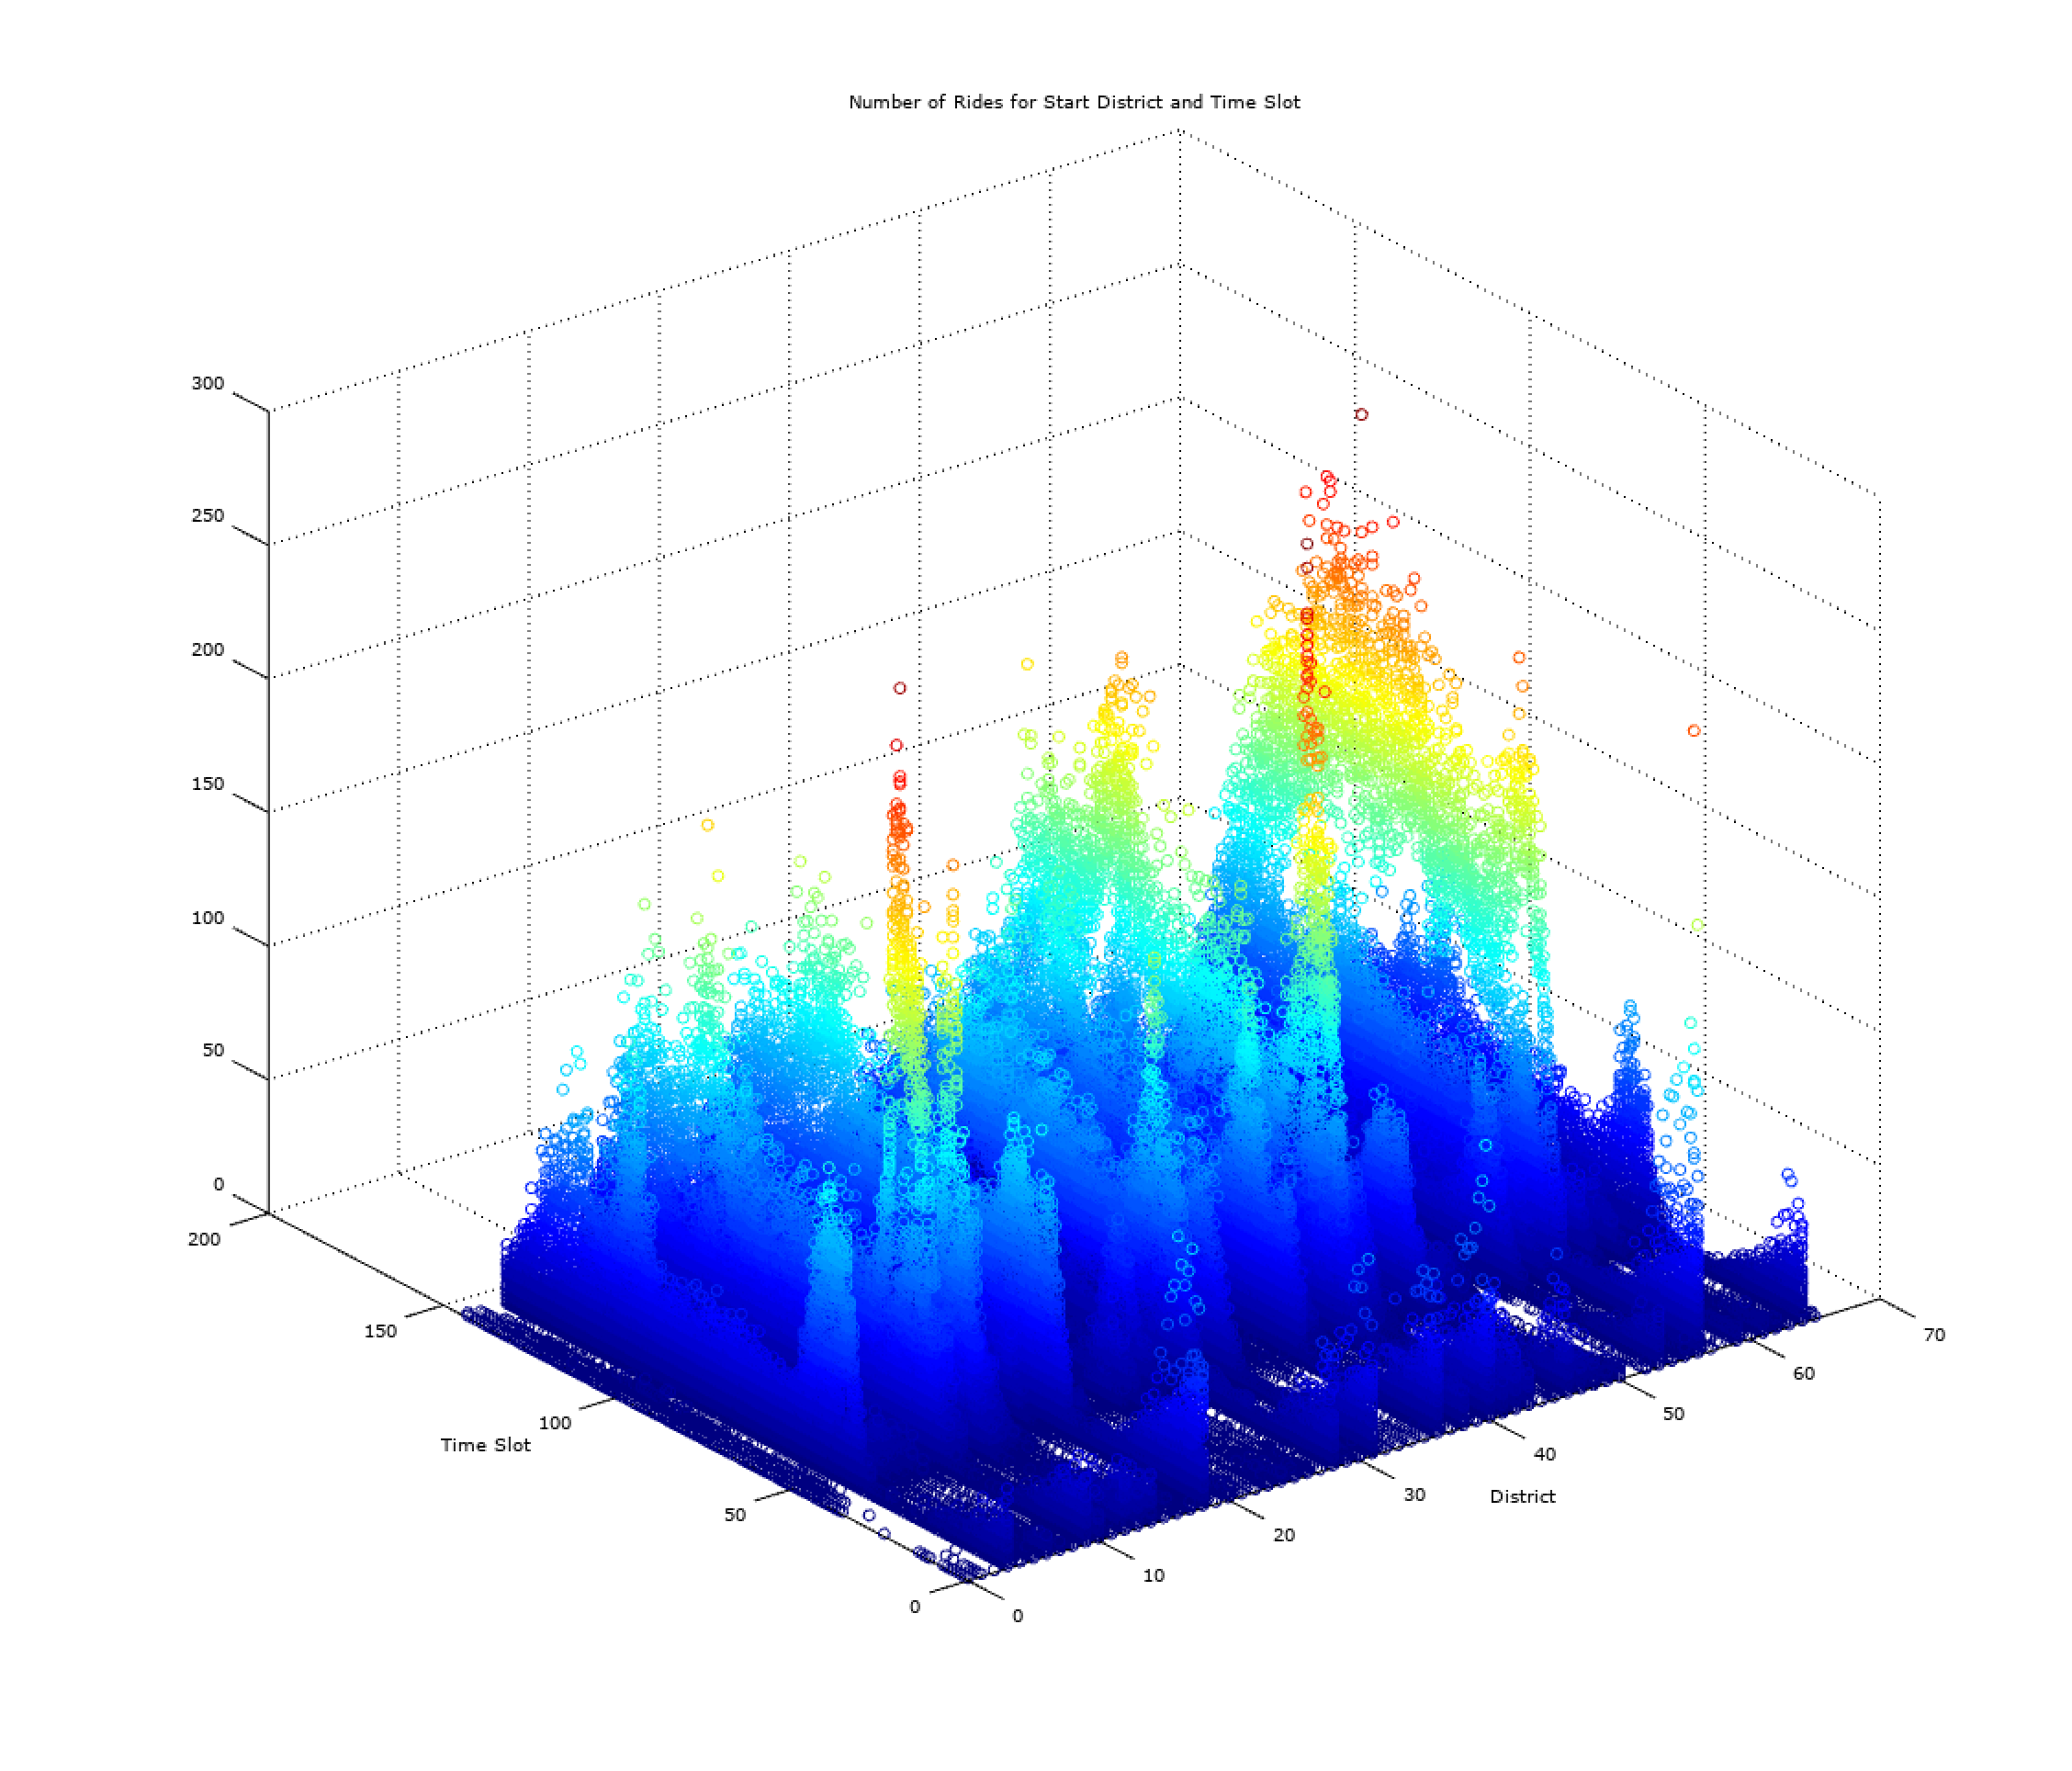
\includegraphics[width=3in]{figures/NumberofRidesforDistrictandTimeSlot.png}
\caption{Number of rides scatter plot for start district and time slot.}
\label{rides3}
\end{figure}

Next we plotted the number of rides and the order price for each data point after it had been projected on the first two eigen vectors and multiplied by the corresponding eigen values. These are shown in figures \ref{rides} and \ref{price}. These plots show that for the same coordinate along the first two eigen vectors, there are many values for the number of rides and price. This is an indication of the complexity of the data and the difficulty in using it to make predictions. The number of rides plot for the start district and day of week in figure \ref{rides2} also shows a similar complexity that makes prediction difficult. Figure \ref{rides3} is another example of data complexity. \\

\begin{figure}[!htb]
\centering
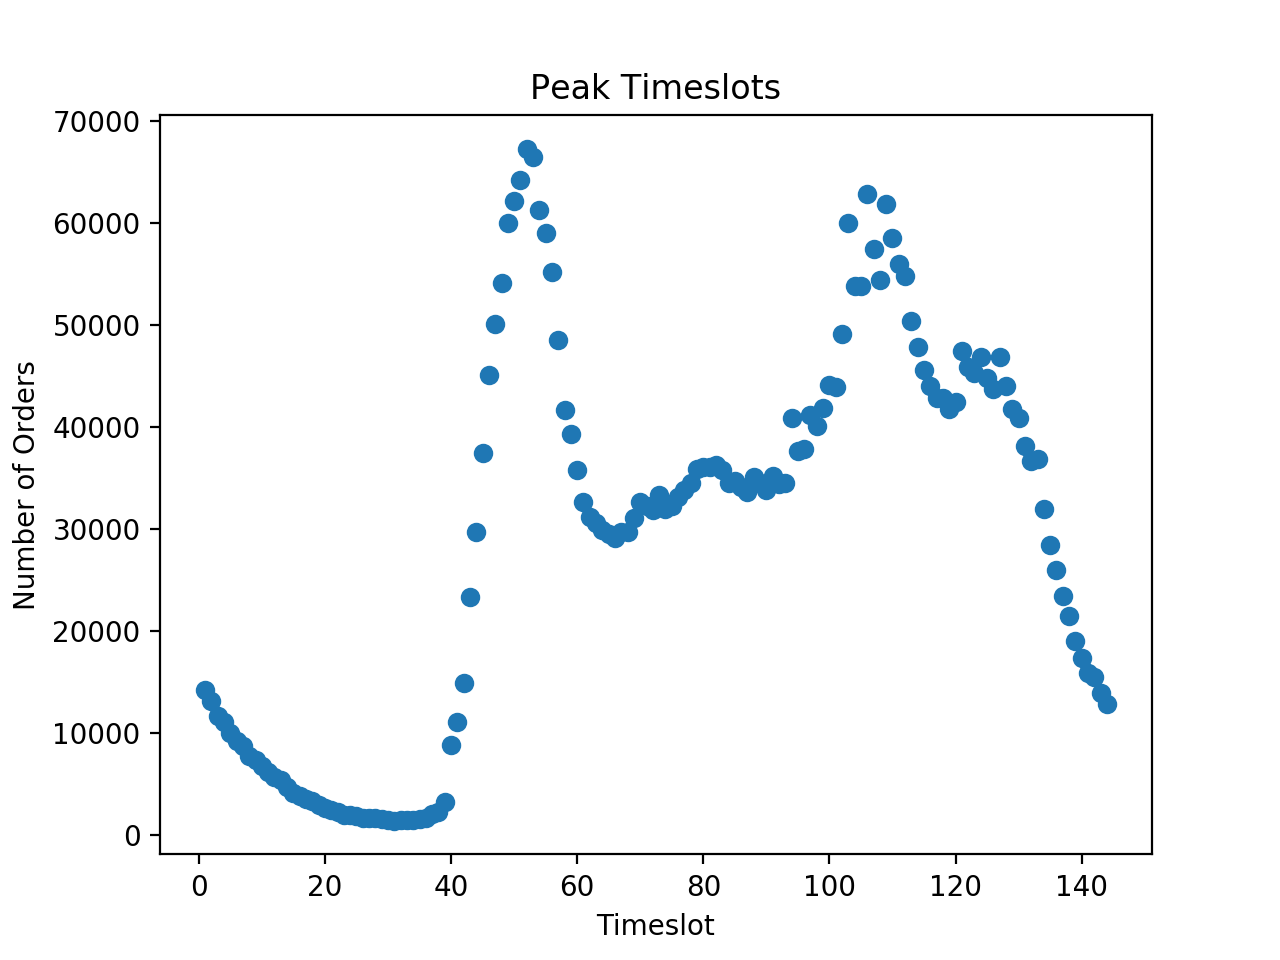
\includegraphics[width=3in]{figures/PeakTimeslots.png}
\caption{Number of rides scatter plot for a timeslot (Monday-Friday).}
\label{peak}
\end{figure}

\begin{figure}[!htb]
\centering
\subfloat{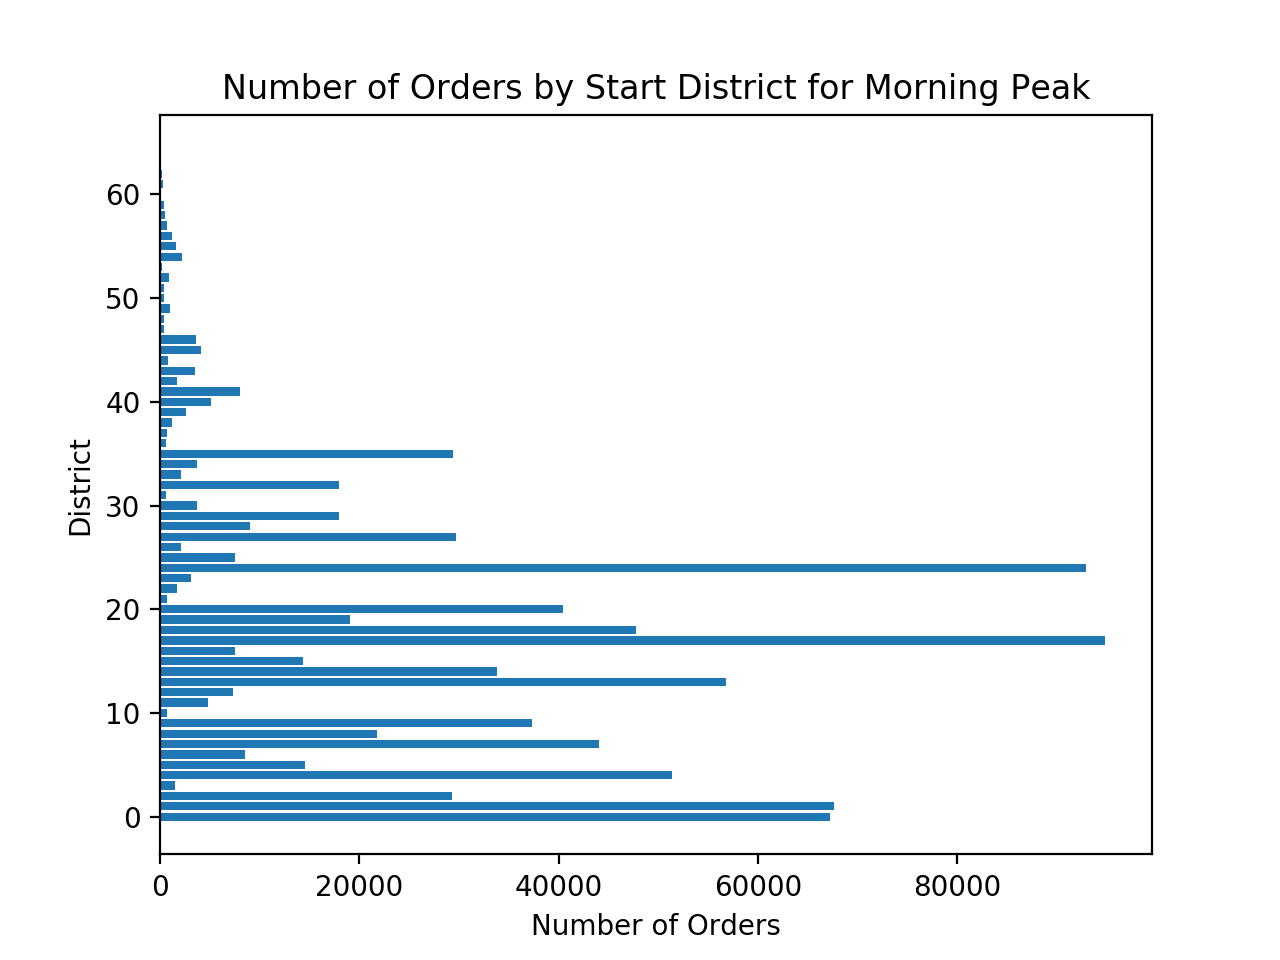
\includegraphics[width=3in]{figures/StartMorning.png}}
\subfloat{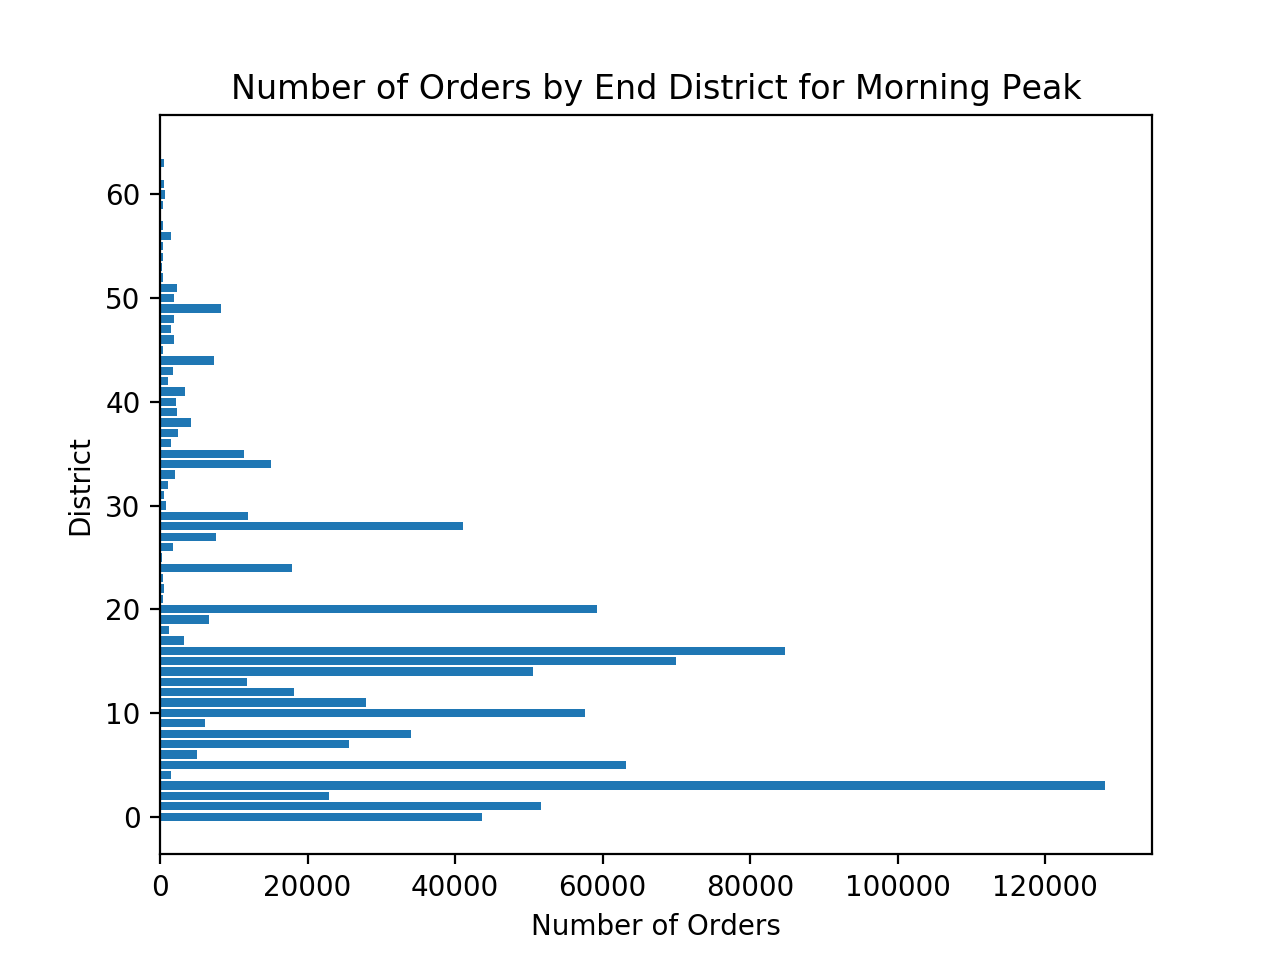
\includegraphics[width=3in]{figures/EndMorning.png}}
\caption{Number of rides scatter plot for a district during peak time period (Monday-Friday).}
\label{peakDistrict}
\end{figure}

We also looked at patterns that could be attributed to the passengers taking taxis to and from work. Using a Monday through Friday work week, we first found the peak timeslots shown in figure \ref{peak}. Then using the peak timeslots, we plotted the number of orders per start district and the number of orders per end district for the first peak shown in figure \ref{peakDistrict}. While there does appear to be some pattern that could lead to deducing residential and commercial districts, the pattern is not strong enough to reduce the complexity of the dataset.\\

The dataset can be separated into different collections, the DateTime collection, the POI collection, the Weather collection, and the Traffic collection. Each collection in the dataset has been expanded to allow for the categorization of the variables. We ran dimension reduction on each collection separately to obtain a two-dimension subspace using Singular Value Decomposition(SVD). The objective of the SVD process was to visualize the collections to determine if the collection will fit to a linear line.  These visualizations further proved that the dataset is not of a linear fit.

%------------------------------------------------
\section{Conclusion}
 
It looks like traditional regression methods do not work for complicated situations where we need to model human behavior. Deep learning techniques have been shown to give better results where traditional methods have failed or do not result in the desired level of accuracy. This is possibly a problem that is better suited to using deep learning.

%----------------------------------------------------------------------------------------
\begin{thebibliography}{1}

\bibitem{DidiPage}
\enquote{Algorithm Competition.} \textit{Algorithm Competition}. N.p., n.d. Web. 28 Jan. 2017.

\bibitem{sklearn}
\enquote{Scikit-learn.} \textit{Scikit-learn: Machine Learning in Python - Scikit-learn 0.18.1 Documentation.} N.p., n.d. Web. 19 Mar. 2017.

\end{thebibliography}

\end{document}